\chapter{Исследовательская часть}

\section{Технические характеристики устройства}

Ниже представлены характеристики компьютера, на котором проводилось тестирование программы:
\begin{itemize}[label=---]
    \item операционная система Windows 10 Домашняя;
    \item оперативная память 12 Гб;
    \item процессор Intel(R) Core(TM) i7-9750H CPU @ 2.6 ГГц.
\end{itemize}

Во время тестирования ноутбук был подключен к сети электропитания. 
Процессор был загружен на 19\%, оперативная память -- на 50\%.


\section{Демонстрация работы программы}
На рисунках \ref{fig:parallel_ex} -- \ref{fig:linear_ex} приведены примеры работы программы конвейерной реализаций и 
линейной реализаций.
\begin{figure}[h]
	\centering
	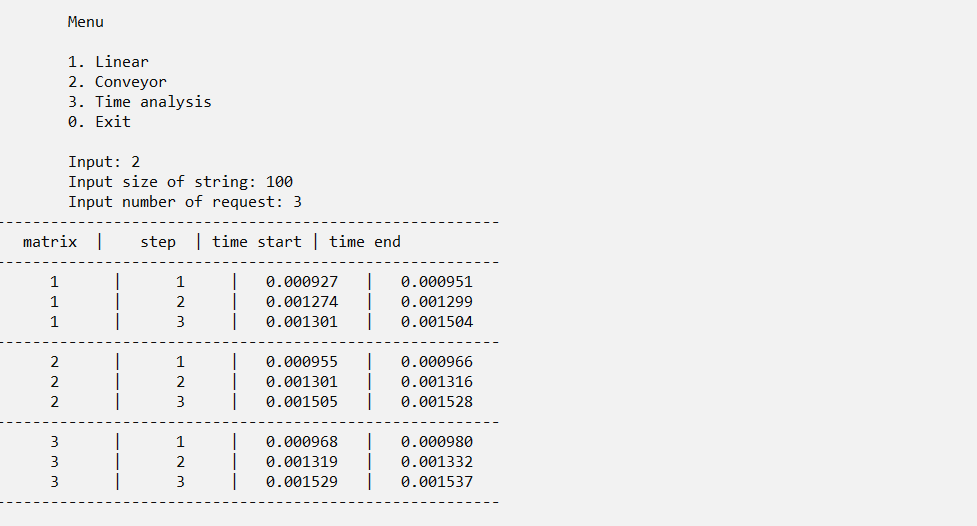
\includegraphics[scale=0.6]{img/example_para.png}
	\caption{Пример работы программы (конвейерная реализация)}
	\label{fig:parallel_ex}
\end{figure}

\begin{figure}[h]
	\centering
	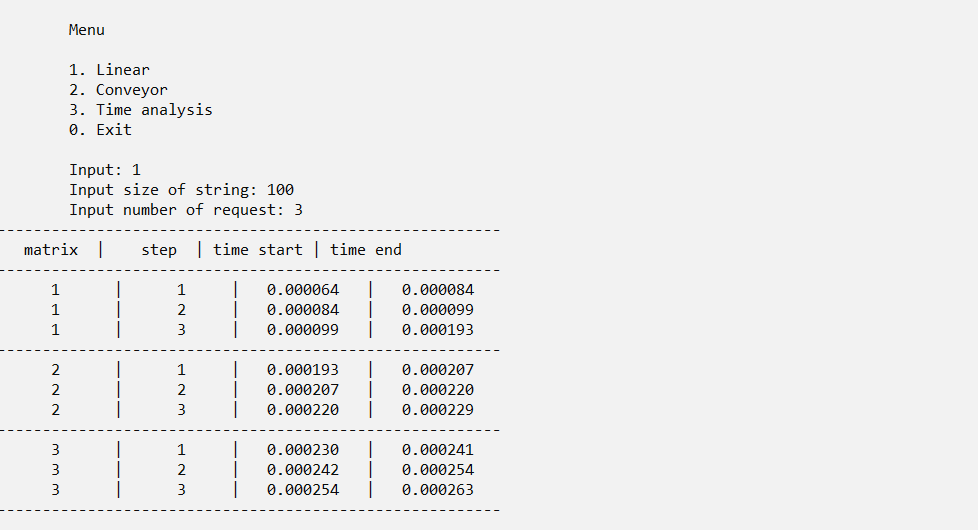
\includegraphics[scale=0.6]{img/example_linear.png}
	\caption{Пример работы программы (линейная реализация)}
	\label{fig:linear_ex}
\end{figure}

\section{Время выполнения алгоритмов}

Чтобы получить достаточно точное значение, производилось усреднение времени. 
Количество запусков замера процессорного времени 1000 раз.

В таблице \ref{tbl:test1} приведены результаты замеров времени работы реализаций линейного и конвейерного алгоритмов c одном размером строки.

\begin{table}[ht]
	\small
	\begin{center}
		\begin{threeparttable}
			\caption{Результаты замеров времени}
			\label{tbl:test1}
			\begin{tabular}{|c|c|c|c|}
				\hline
				\bfseries Размер строки & \bfseries Кол--во строки & \bfseries Линейный& \bfseries Конвейерный
				\csvreader{csv/4patok.csv}{} 
				{\\\hline \csvcoli & \csvcolii & \csvcoliii & \csvcoliv} \\
				\hline
			\end{tabular}	
		\end{threeparttable}
	\end{center}
\end{table}

\clearpage
В таблице \ref{tbl:test2} приведены результаты замеров времени работы реализаций линейного и конвейерного алгоритмов c одном количеством строки.

\begin{table}[ht]
	\small
	\begin{center}
		\begin{threeparttable}
			\caption{Результаты замеров времени}
			\label{tbl:test2}
			\begin{tabular}{|c|c|c|c|}
				\hline
				\bfseries Размер строки & \bfseries Кол--во строки & \bfseries Линейный& \bfseries Конвейерный
				\csvreader{csv/manypatok.csv}{} 
				{\\\hline \csvcoli & \csvcolii & \csvcoliii & \csvcoliv} \\
				\hline
			\end{tabular}	
		\end{threeparttable}
	\end{center}
\end{table}


\section{Вывод}

В этом разделе были указаны технические характеристики машины, на которой происходило сравнение времени работы алгоритмов обработки строк для конвейерной и ленейной реализаций.

В результате замеров времени было установлено, что конвейерная реализация обработки лучше линейной при большом количестве строк (в 3 раза при 400 строки, 800 и 1600). 
Так же конвейерная обработка показала себя лучше при увеличении размеров обрабатываемых строк (в 5 раза при размере строки 160 и 320). 
Значит при большом количестве обрабатываемых строк, а также при обработке строки большого размера стоит использовать конвейерную реализацию обработки, а не линейную.


